%% The following is a directive for TeXShop to indicate the main file
%%!TEX root = diss.tex

\chapter{A Taxonomy of 3D Reconstruction}
\label{ch:3DRecon_Taxo}
Existing taxonomies of 3D reconstruction techniques generally classify algorithms based on algorithmic details: the survey on Multi-view Stereo algorithms uses taxonomies that differentiate the key properties of each algorithm~\cite{seitz2006comparison}. Reviews of Structured Light techniques typically classify techniques based on the type of projection pattern used~\cite{geng2011structured, salvi2004pattern}. Photometric Stereo algorithms are classified by the assumptions or generalizations made, such as, unknown/known reflectance, unknown/known light conditions (uncalibrated/calibrated), and so on~\cite{shi2016benchmark}. These frameworks provide a way to categorize intra-category algorithms, but are unsuitable to compare the performance of inter-category algorithms. Furthermore, the algorithms under consideration target limited categories of objects. It is well known that such algorithms are highly likely to fail when targeting a diverse set of object categories. Thus, it is crucial to understand where algorithms perform well and where they fail when designing an application for reconstruction. Under the previous framework of taxonomy, this knowledge is largely empirical, with each algorithm mapped roughly to a sub-volume in the problem space that is poorly defined. To overcome this limitation, we take a more \textit{object-centered approach} instead of an \textit{algorithm-centered approach}.

The taxonomy proposed in this chapter defines 3D reconstruction techniques from an object-centered viewpoint, \ie categorizes an algorithm based on the class of objects that it can reliably work under. This taxonomy transforms the 3D reconstruction problem from one requiring knowledge and expertise of specific algorithms in terms of \textit{how} to use them, to one requiring knowledge of working conditions of each algorithm.

\section{A New Perspective of Taxonomy}
Typical taxonomies are algorithm centric, describing and classifying algorithms based on \textit{how} an algorithm solves the problem. However, this approach gives very little insight to the conditions that allow a specific algorithm to work well. Further, it requires vision knowledge to understand and use these algorithms. The new perspective approaches taxonomy from a different angle, more specifically, the algorithms are categorized based on the type of objects/problem conditions that they can reliably work under. We first give an overview of object classes, which serves as the bases to the taxonomy, then proceeds to investigate the working conditions of each class of algorithms based on reports in relevant literature.

\subsection{Object class}
In Figure~\ref{fig:obj_class}, we show a taxonomy of object classes with different material and shape properties. However, by no means are these presented object classes complete. There are many other properties not included that are commonely seen in the real world. For instance, effects such as occlusion, discontinuity, and emission, among others, are not considered. The rationale behind our choice is that most techniques that have been developed over the past few decades mainly tackle object with an opaque and diffuse surface. For specular, refractive, and translucent or transparent objects, only very specialized algorithms are applicable for reconstruction~\cite{ihrke2010transparent}. To approach this problem in a feasible manner, six classes of objects are being investigated in depth. They are selected based on the availability of reliable techniques and the diversity of corresponding real-world objects. We propose the following labels to differentiate object classes. For each class label, the properties are ordered as follows: translucency, texture, lightness, reflection model, surface roughness, and concavity. See the six classes of objects in Table~\ref{tab:six_obj_class}.
\begin{figure}[!htbp]
\centering
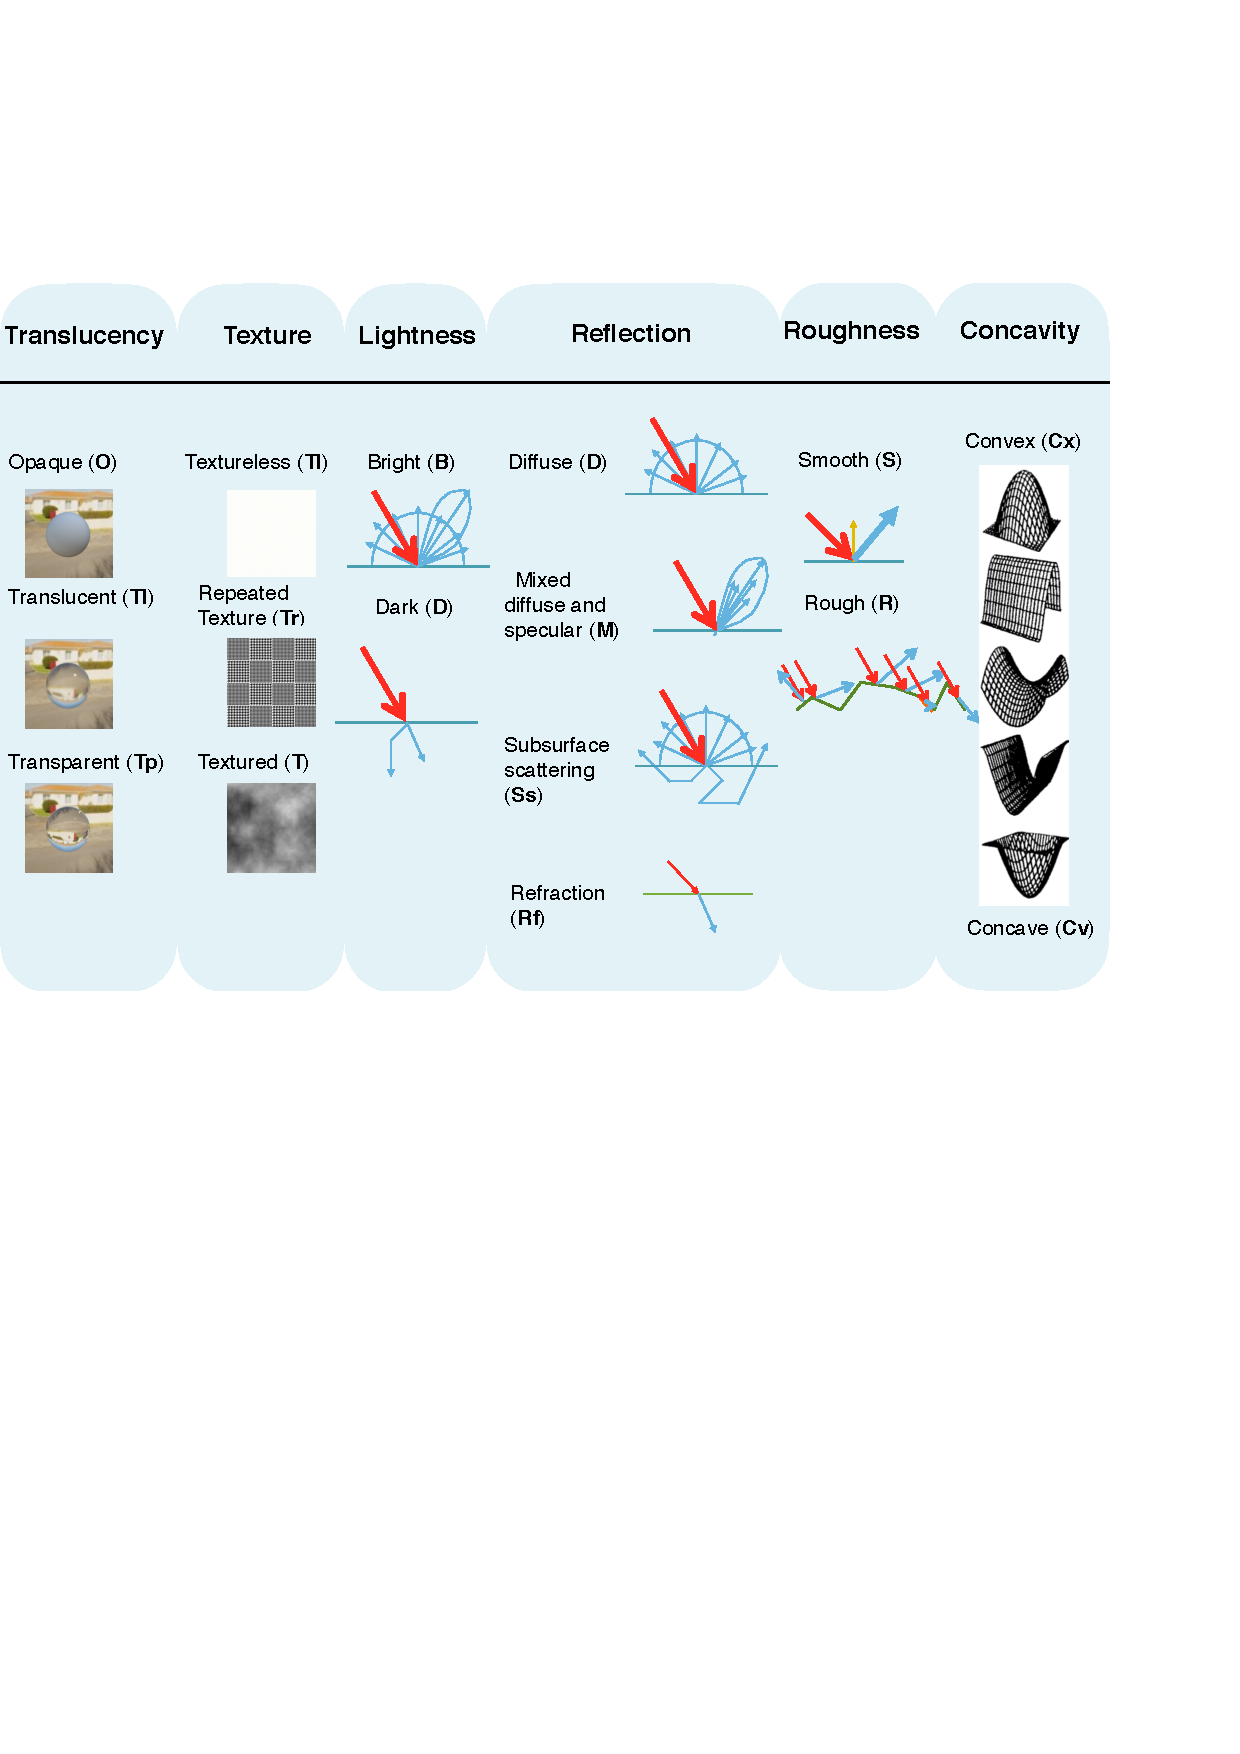
\includegraphics[width=\textwidth]{taxo/obj_class}\\
\caption{A list of properties for object classes.}
\label{fig:obj_class}
\end{figure}

\subsubsection{Class labels}
\begin{itemize}
\item \textbf{Translucency}: \textbf{O}: opaque, \textbf{Tl}: translucent, \textbf{Tp}: transparent.
\item \textbf{Texture}: \textbf{T}: textured, \textbf{Tr}: repeated textured, \textbf{Tl}: textureless.
\item \textbf{Lightness}: \textbf{B}: bright, \textbf{D}: dark.
\item \textbf{Reflection}: \textbf{D}: diffuse model, \textbf{S}: specular model, \textbf{M}: mixture of diffuse and specular, \textbf{Ss}: subsurface scattering, \textbf{Rf}: refraction
\item \textbf{Roughness}: \textbf{S}: smooth, \textbf{R}: rough
\item \textbf{Concavity}: \textbf{Cx}: convex, \textbf{Cv}: concave
\end{itemize}

\begin{table}[!htbp]
\centering
\begin{tabular}{ll|l}
\toprule
Class \# & Description & Label\\
\midrule
1 & Textureless, bright, diffuse reflectance & O-Tl-B-D-R-Cx\\
2 & Textureless, bright, mixed reflectance & O-Tl-B-M-S-Cx\\
3 & Textured, bright, diffuse reflectance & O-T-B-D-R-Cx\\
4 & Textured, bright, mixed reflectance & O-T-B-M-S-Cx\\
5 & Textured, dark, diffuse reflectance & O-T-D-D-S-Cx\\
6 & Textured, dark, mixed reflectance & O-T-D-M-S-Cx\\
\bottomrule
\end{tabular}
\caption{Label of six classes of objects.}
\label{tab:six_obj_class}
\end{table}

\subsubsection{A traditional taxonomy}
Traditionally, algorithms are categorized into different classes based on the visual cues used for reconstruction, as discussed in Chapter~\ref{ch:RelatedWork}. 
Table~\ref{tab:class_algo} gives an example of what a typical taxonomy would look like.
\begin{table}[!htbp]
  \centering
  \begin{tabular}{l|l}
  \toprule
  \textbf{Algo. class} & \textbf{Technique}\\
  \midrule
  SfS & Horn~\cite{horn1970shape}\\
  MVS & Furukawa~\cite{furukawa2010accurate}, Goesele~\cite{goesele2006multi}, Vogiatzis~\cite{vogiatzis2007multiview}, \\
      & Hern{\'a}ndez~\cite{esteban2004silhouette}, Faugeras~\cite{faugeras2002variational}\\
  Lamberian PS & Woodham~\cite{woodham1980photometric}, Hayakawa~\cite{hayakawa1994photometric}, Belhumeur~\cite{belhumeur1999bas}, \\
      & Alldrin~\cite{alldrin2007resolving}\\
  Non Lambertian PS & Coleman~\cite{coleman1982obtaining}, Barsky~\cite{barsky20034}, Schluns~\cite{schluns1993photometric}, Sato~\cite{sato1994temporal}, \\
      & Mallick~\cite{mallick2005beyond}, Alldrain~\cite{alldrin2008photometric}, Goldman~\cite{goldman2010shape}, Silver~\cite{silver1980determining}, \\
      & Hertzmann~\cite{hertzmann2005example}, Zickler~\cite{zickler2002helmholtz}\\
  % MVPS & \checkmark & \\
  SL & Inokuchi~\cite{inokuchi1984range}\\
  VH & Szeliski~\cite{szeliski1993rapid}, Matusik~\cite{matusik2002efficient}, Tarini~\cite{tarini2002marching}\\
  \bottomrule
  \end{tabular}
  \caption{A traditional taxonomy that classifies algorithms based on algorithmic details.}
  \label{tab:class_algo}
\end{table}

\section{Working conditions of algorithms}
This section investigates the cases where each category of algorithms is capable of working under based on the reported literature. Only visual texture is considered, and it can be thought of as a pattern or variance of intensity appearing on an object's surface. In this thesis, the visual texture will be considered as resulting from non-uniform surface albedo. Thus, uniform albedo represents uniform texuture while non-uniform albedo represents textured surfaces.

\subsection{Multi-view Stereo}
The working conditios of Multi-view Stereo algorithms are summarized in Table~\ref{tab:mvs_cond}. For a typical MVS algorithm to perform well, the object should have a textured and diffuse surface.

\subsubsection{High texture}
Multi-view Stereo algorithms take advantage of textural information to establish point correspondences across different views. Thus homogeneous surfaces pose great challenges to MVS algorithms. However, some MVS algorithms tested on a textureless object ``Dino'' in the Middlebury MVS benchmark~\cite{seitz2006comparison} give successful reconstruction results. This demonstrates that MVS algorithms are able to exploit very weak and intricate image textures, most of which come from shading and/or shadowing effects. However, these texture are so weak that images need to have very high quality.

% \citeauthor{furukawa2008high} use wide-baseline stereo matching to recover the 3D coordinates of salient feature points, then shrink a visual hull model so that the recovered points lie on its surface, then refine the result using energy minimization. \citeauthor{goesele2006multi} compute a depth map from each camera viewpoint (similar to [31]) and merge the results using VRIP [62]. \citeauthor{esteban2004silhouette} first compute a depth map from each camera viewpoint and merge the results into a cost volume. They then iteratively deform a mesh, initialized at the visual hull, to find a minimum cost surface in this volume, also incorporating terms to fit silhouettes. Kolmogorov and Zabih [35] compute a set of depth maps using multi-baseline stereo with graph cuts, then merge the results into a voxel volume by computing the intersections of the occluded volumes from each viewpoint. \citeauthor{faugeras2002variational} compute a minimum cost surface by evolving a surface in a level-set frame-work, using a prediction-error measure. \citeauthor{vogiatzis2007multiview} compute a correlation cost volume in the neighborhood of the visual hull. A minimum-cost surface is then computed using volumetric min-cut.

\subsubsection{Diffuse reflectance}
Most MVS algorithms require that the object surface with similar or same appearances from different perspectives, and hence, most of the algorithms assume Lambertian reflectance. While pure Lambertian surfaces are rare in reality, it is empirically verified that MVS algorithms perform reasonably well on non-Lambertian surfaces. As long as the cameras can capture the diffuse reflectance component, and then the photo-consistency function is able to identify and ignore images whose non-diffsue effects (e.g., specular highlights) are strong, then utilize the diffuse component in the remaining images. Further, there are some attempts to overcome this limitation, a pure passive methods was proposed that directly model and analyze non-Lambertian effects for MVS algorithms~\cite{jin2003multi,jin2005multi}.
\begin{table}[!htbp]
  \centering
  \begin{tabular}{l*{5}{p{15mm}}}
  \toprule
  \textbf{Technique} & Texture & Lightness & Reflectance & Roughness & Concavity\\
  \midrule
  MVS & Textured & - & Diffuse or mixed & - & -\\
  \bottomrule
  \end{tabular}
  \caption{Working condition of Multi-view Stereo algorithms.}
  \label{tab:mvs_cond}
\end{table}

\subsection{Shape from Shading}
Shape from Shading, first proposed by Horn~\cite{horn1970shape}, specifically targets isotropic, known Lambertian surfaces. By assuming orthographic projection, and known light source intensity and direction, surface orientation can be estimated from shading variations. The working condition is shown in Table~\ref{tab:sfs_cond}.

\subsubsection{Reflectance model}
Though other reflectance models are feasible, typical SfS algorithms assume Lambertian reflectance model. The reason is that surface lightness is directly related to surface orietation and reflectance model once the light source and viewing direction are fixed. This is generally an ill-posed problem even with the simplest reflectance model since there is only one intensity value per pixel to solve for surface orientation, which has two DoF. However, even in the simplest case, the survey by Zhang~\cite{zhang1999shape} demonstrate that SfS algorithms generally perform poorly, and none performs well in all cases.

\subsubsection{Interreflection}
Typical SfS algorithms cannot deal with interreflections, since the surface lightness would be corrupted by light transport between surface facets. Thus, object exhibit any form of concavity will pose great challenge to SfS algorithms.

\begin{table}[!htbp]
  \centering
  \begin{tabular}{l*{5}{p{15mm}}}
  \toprule
  \textbf{Technique} & Texture & Lightness & Reflectance & Roughness & Concavity\\
  \midrule
  SfS & Textureless & Bright & Lambertian & Smooth & Convex\\
  \bottomrule
  \end{tabular}
  \caption{Working condition of Shape from Shading algorithms.}
  \label{tab:sfs_cond}
\end{table}

\subsection{Photometric Stereo}
Photometric Stereo can be considered as an extension of SfS algorithms, which adds additional light sources to remove the ambiguity faced by SfS algorithms. The working conditions of Photometric Stereo algorithms are summarized in Table~\ref{tab:ps_cond}.

\subsubsection{Albedo}
Photometric Stereo algorithms work more reliably on surfaces with sufficiently strong albedo. This is because the algorithm exploits the intensity variation as a visual cue, which is more challenging to detect on surfaces with low intensity values.

Though SfS algorithms requires uniform albedo, typical PS algorithms can be used easily on surfaces with spatially varying albedo. First the albedo-scaled normal can be estimated, then the albedo is retrieved as the magnitude of the scaled normal~\cite{woodham1980photometric}.

\subsubsection{Lambertian reflectance model} % Lambertian PS: uniform reflectance
The Lambertian PS algorithms can be divided into two groups: calibrated, and uncalibrated method. The original PS proposed by Woodham~\cite{woodham1980photometric} can be considered as calibrated Lambertian PS. Later, more uncalibrated Lambertian PS have been proposed to avoid this tedious process.

Silver~\cite{silver1980determining} proposed a look-up scheme that relies on a reflectance object with the same reflectance as the target, which in this case is a uniform Lambertian surface. This approach is later adapted to surface with non-Lambertian reflectance with varying albedo or material in~\cite{hertzmann2005example}.

Another successful uncalibrated approach used six or more pixels with the same albedo, and was able to solve for normals up to a rotation ambiguity\cite{hayakawa1994photometric}. It can be further proved that a 3-parameter subset of these transformations, known as the Generalized Bas-Relief (GBR) ambiguity, preserve surface integrability~\cite{belhumeur1999bas}. Thus, given three or more imges of a Lambertian object acquired under light sources of unknown direction and strength, the surface can be reconstructed up to GBR transformation by enforcing surface integrability, see Figure~\ref{fig:gbr} for the effect of GBR-ambiguity.
\begin{figure}[!htbp]
\centering
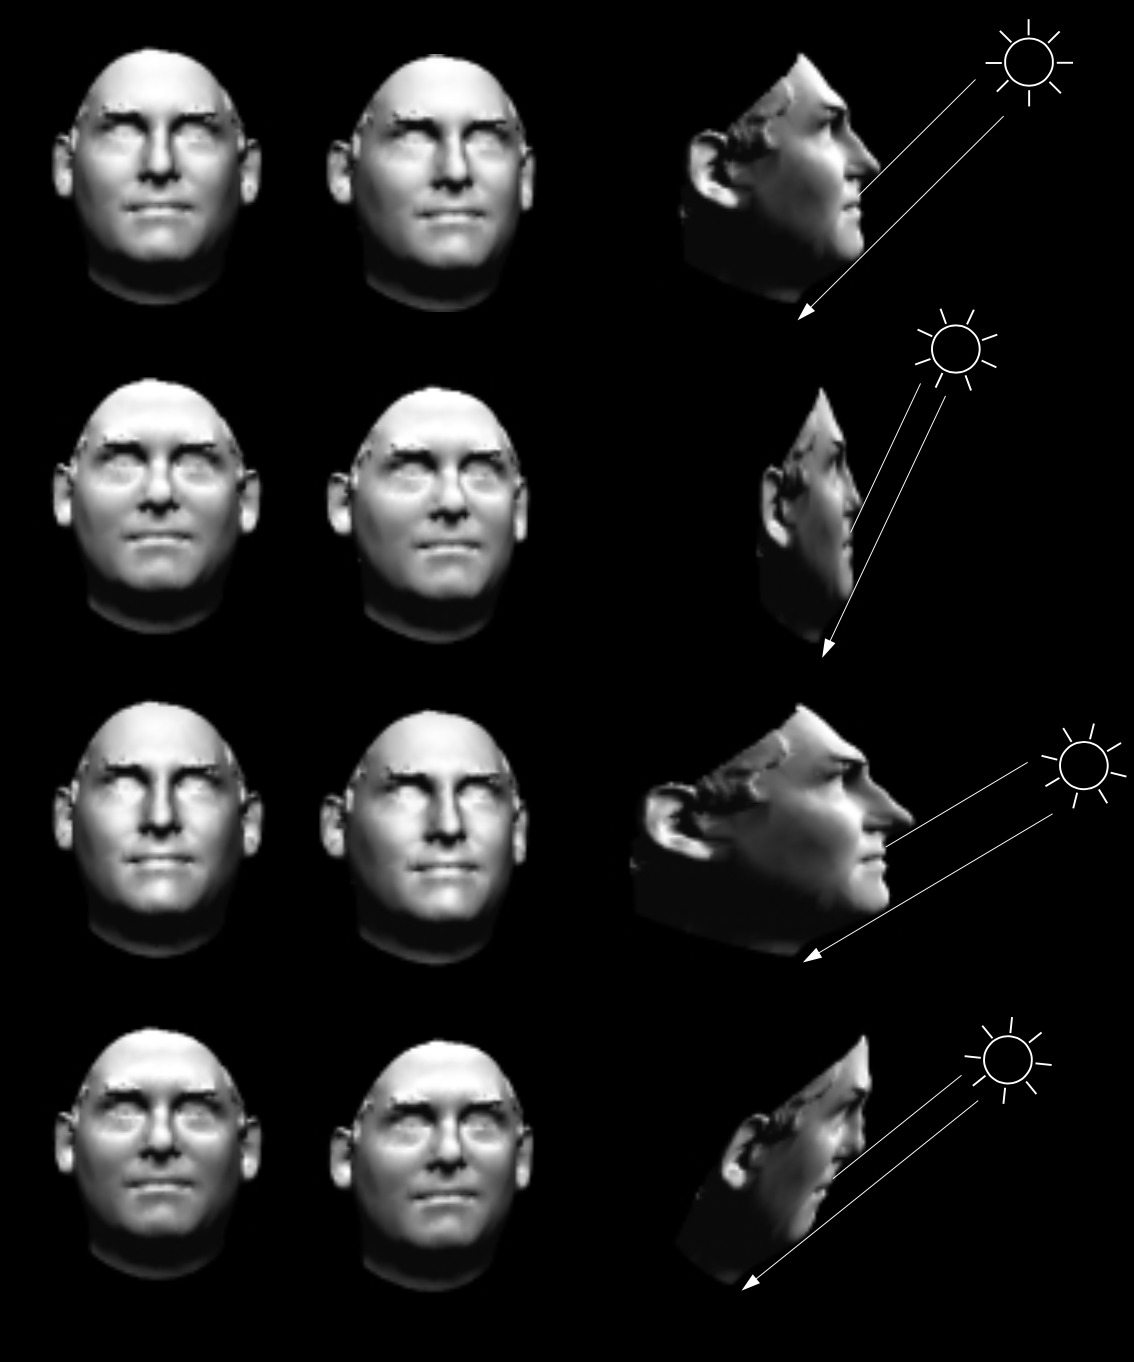
\includegraphics[width=0.6\textwidth]{taxo/gbr.png}
\caption{The effect of GBR ambiguity. Two sets of shape and light source configurations can produce exactly the same images.}
\label{fig:gbr}
\end{figure}

\subsubsection{Non-Lambertian reflectance model}
Much of the emphasis in PS has been to relax the assumption of Lambertian reflectance. There are four classes of Non-Lambertian PS algorithms: the first class treats specular component as outliers~\cite{coleman1982obtaining,barsky20034,ikeuchi1981determining,nayar1990determining}; the second class uses reference object that has the same material as the target object~\cite{hertzmann2005example}; the third class assumes that the reflectance can be modeled as a linear combination of a set of basis reflectance models~\cite{goldman2010shape,alldrin2008photometric}; and the fourth class exploits the physical properties common to large classes of BRDFs, such as energy-conservation, non-negativity, Helmholtz reciprocity, isotropy, and so on~\cite{zickler2002helmholtz,tan2007isotropy,alldrin2007toward}.

% One line of approaches exploit the observation that the reflectance of many material can be approximated by the sum of a specular and a diffuse lobe.
% The \textit{reference object} approach, first proposed by~\citeauthor{silver1980determining}, and later revisited by in~\cite{hertzmann2005example}, can be used for surfaces with spatially varying reflectance. The basic assumption is that the BRDF at each point is a linear combination of the ``basis'' BRDFs defined by the set of reference objects.

% One approach exploits the fact that the reflectance of non-Lambertian surfaces can be approximated by \textbf{diffuse component and specular lobe}. \citeauthor{coleman1982obtaining} and \citeauthor{barsky20034} who treat specular pixels as outliers, and \citeauthor{schluns1993photometric}, \citeauthor{sato1994temporal}, and \citeauthor{mallick2005beyond} who assume the color of the specular lobe differs from the color of the diffuse lobe, allowing separation of the specular and diffuse components.

% Due to the high complexity of the BRDF, some methods utilize {analytical reflectance models}. \citeauthor{goldman2010shape} uses an isotropic Ward model for each basis BRDF, and the surface orientation and parameters of the reflectance models are estimated iteratively. \citeauthor{alldrin2008photometric} proposed a data-driven approach that got rid of the parametric reflectance model, and employed an novel bi-variate approaximations of isotropic reflectance functions. By combining this approximation with the weighted basis BRDFs, a per-pixel surface normal, global set of non-parametric basis BRDFs, and the corresponding weights are able to be independently estimated. Though the parametric reflectance model can significantly reduce the complexity of BRDFs, they are typically restricted to a limited classes of materials.

% Another alternative to using BRDF models is to take advantage of the properties of BRDFs, include energy conservation, non-negativity, Helmholtz reciprocity, or isotropy. Helmholtz stereopsis introduced by~\citeauthor{zickler2002helmholtz} exploits the reciprocity to obtain the surface reconstruction. Isotropy is another physical property which holds for material without ``grain''. \citeauthor{tan2007isotropy} use both symmetry and reciprocity present in isotropic BRDFs to resolve the generalized bas-relief ambiguity. \citeauthor{alldrin2007toward} show that isotropy, with no further assumptions on surface shape or BRDF, can be utilized to recover the surface normal at each surface point up to a plane.

% A four-source photometric stereo technique uses a fourth source of illumination to detecta and remove specular reflections~\cite{coleman1982obtaining}. By adding a fourth image, it's possible to compute four sets of normals, \ie one normal for each permutation of three intensity values. If there is a greater deviation in both magnitude and direction of the normals, a method can now be developed to eliminate specular effects using a thresholding procedure.

\subsubsection{Convexity}
Active methods that assumes a local reflectance model such as most PS algorithms can work more reliably on surfaces without casting shadow and interreflection. Thus surfaces with concavities pose a great challenge for this type of techniques since the indensity can be affected by other surface patches.

\begin{table}[!htbp]
  \centering
  \begin{tabular}{p{3cm}*{5}{p{15mm}}}
  \toprule
  \textbf{Technique} & Texture & Lightness & Reflectance & Roughness & Concavity\\
  \midrule
  Lambertian PS, uniform albedo & Textureless & Bright & Lambertian & - & Convex\\
  Lambertian PS, non-uniform albedo & Textured & Bright & Lambertian & - & Convex\\
  Non-Lambertian PS & - & Bright & Mixed & - & Convex\\
  \bottomrule
  \end{tabular}
  \caption{Working conditions of typical Photometric Stereo algorithms.}
  \label{tab:ps_cond}
\end{table}

\subsection{Structured Light}
For stereo correspondence based methods, actively projected patterns have to be used for the lack of surface texture. Since the surface is diffuse, there is no specular reflection to cause severe noise. Refer to Table~\ref{tab:sl_cond} for the working condition of SL.

\subsubsection{High albedo}
Regardless of what projection pattern is used, the most important feature of most SL techniques is that it should be able to determine if a surface point is lit or not. Thus, the surface albedo needs to be strong enough so that sufficient amount of reflected light can reach the camera sensor.

\subsubsection{Diffuse reflectance model}
Traditional Structured Light techniques cannot deal with highly specular surfaces since the specular area will exhibit strong reflection even for low lighting conditions, which will cause errors in the encoding process.

\subsubsection{Concexity}
Active methods that assumes a local reflectance model such as most SL algorithms can work more reliably on surfaces without casting shadow and interreflection. Thus surfaces with concavities pose a great challenge for this type of techniques since the indensity can be affected by other surface patches.
\begin{table}[!htbp]
  \centering
  \begin{tabular}{c*{5}{p{15mm}}}
  \toprule
  \textbf{Technique} & Texture & Lightness & Reflectance & Roughness & Concavity\\
  \midrule
  Structured Light & - & Bright & Lambertian & - & Convex\\
  \bottomrule
  \end{tabular}
  \caption{Working condition of typical Structured Light algorithms.}
  \label{tab:sl_cond}
\end{table}

\subsection{Visual Hull}
Visual Hull algorithms don't rely on material properties as long as the foreground of the image can be reliably segmented, thus is applicable for objects with arbitrary visual properties. However, it fails to carve the concavities on the object surface, thus is unsuitable to concave objects.
\begin{table}[!htbp]
  \centering
  \begin{tabular}{c*{5}{p{15mm}}}
  \toprule
  \textbf{Technique} & Texture & Lightness & Reflectance & Roughness & Concavity\\
  \midrule
  VH & - & - & - & - & Convex\\
  \bottomrule
  \end{tabular}
  \caption{Working condition of typical Visual Hull algorithms.}
  \label{tab:ps_cond}
\end{table}
% \begin{table}[!htbp]
%   \centering
%   \begin{tabular}{l*{2}{c}}
%   \hline
%   \textbf{Technique} & Representation & Algorithm\\
%   \hline
%   Szeliski~\cite{szeliski1993rapid} & 3D grids & Voxel-based\\
%   Tarini~\cite{tarini2002marching} & 3D rays & MI-based\\
%   Matusik~\cite{matusik2002efficient} & Polygonal mesh & Exact polyhedral methods\\
%   \hline
%   \end{tabular}
%   \caption{Summary of VH representations and reconstruction approach.}
%   \label{tab:summary_class_6}
% \end{table}

\section{Summary}
Our taxonomy categorizes algorithms based on the problem conditions that they can reliably work under. The problem conditions consists of various visual and geometric properties, as shown in Figure~\ref{fig:obj_class}. These properties can be conceptualized as dimensions of the 3D reconstruction problem space. This taxonomy provides an abstraction which allows us to think of algorithms as volumes within a $n-$dimensional problem space. Existing algorithms can be introduced into this framework based on the performance within the problem space. The aforementioned analysis provide an initial mapping of the space that is summarized below in Figure~\ref{fig:six_class}, and more in detail in Table~\ref{tab:algo_taxo}.
\begin{figure*}[!htbp]
\centering
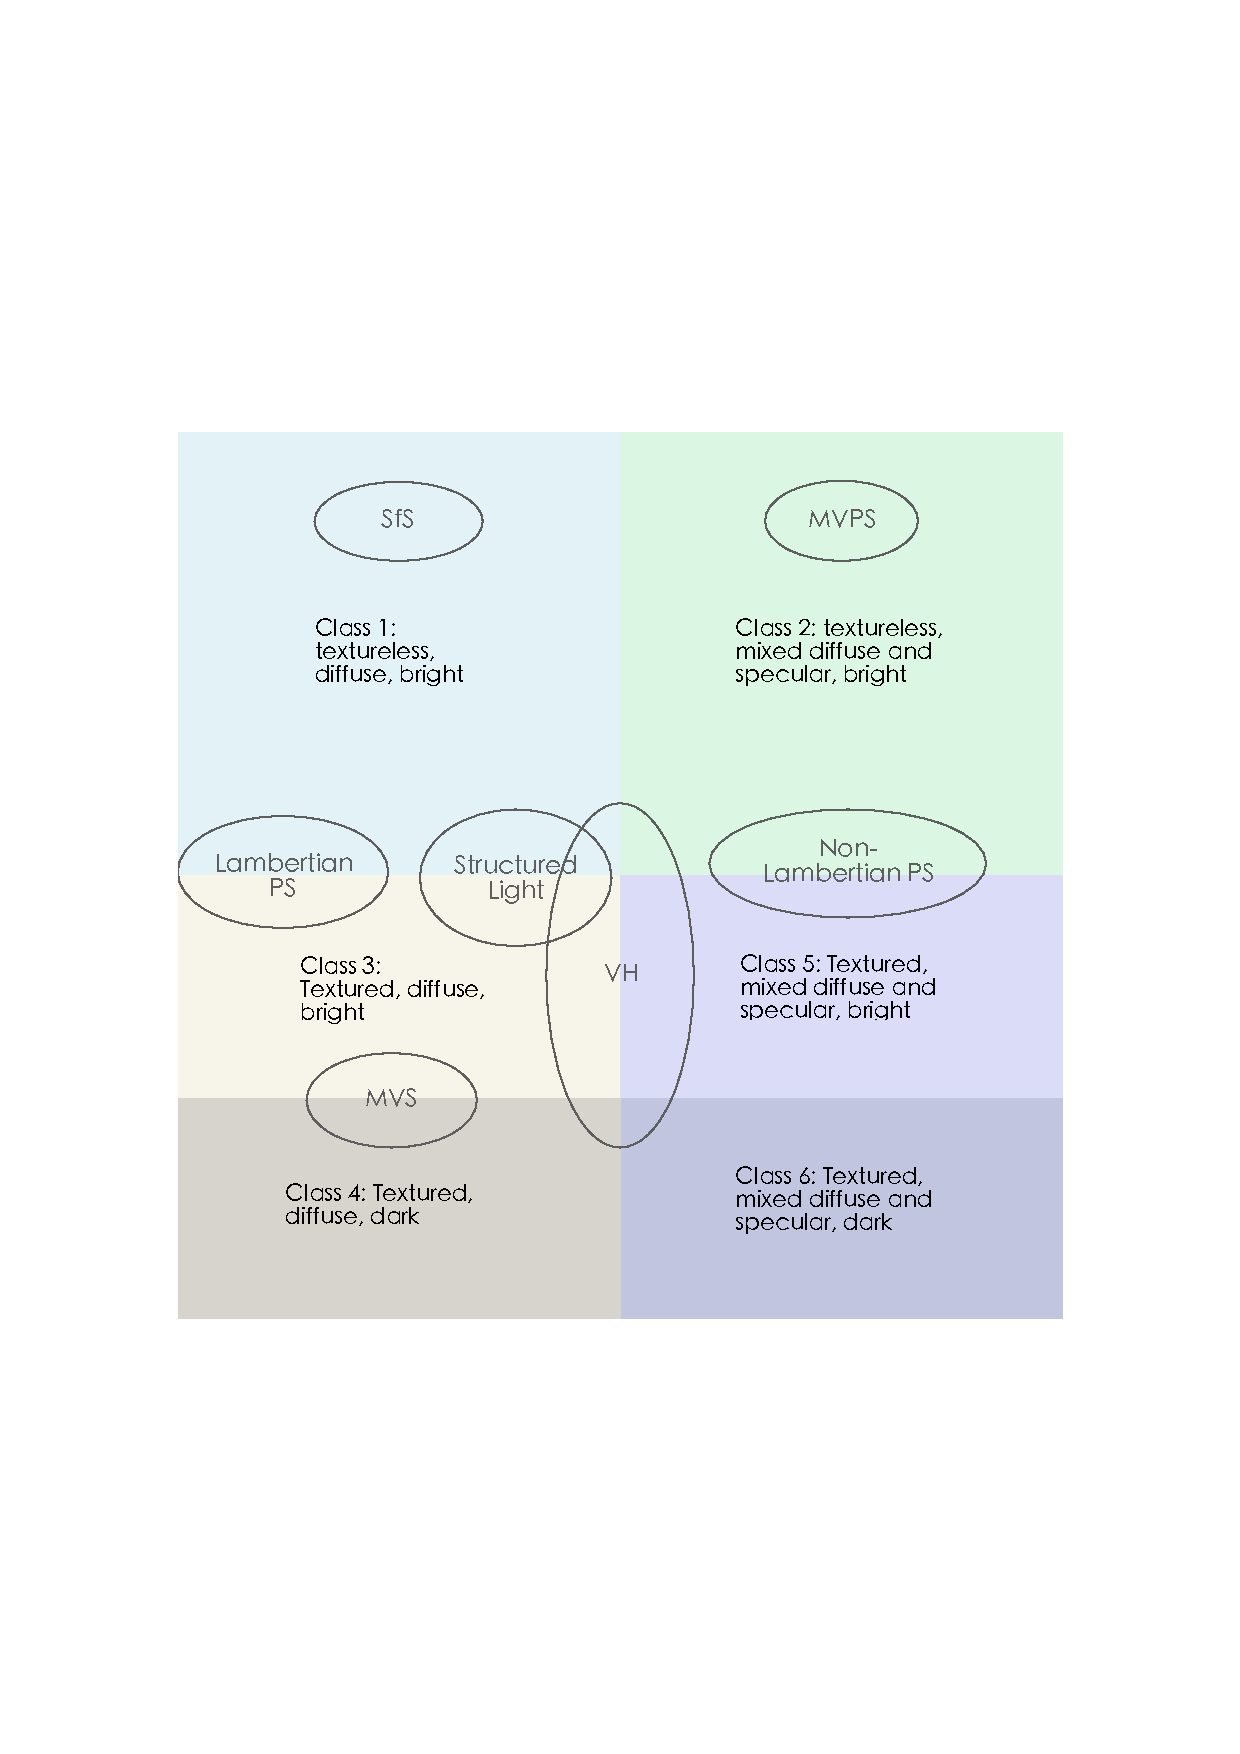
\includegraphics[width=0.5\textwidth]{taxo/six_class}
\caption{Six classes of objects of interest, and the algorithms that could work reliably for these classes.}
\label{fig:six_class}
\end{figure*}

\begin{table}[!htbp]
  \centering
  \begin{tabular}{l|l|p{10cm}}
  \toprule
  \textbf{Class \#} & Class label & Algorithms\\
  \midrule
  1 & \textbf{OTlBDRCx} & Horn~\cite{horn1970shape}, Woodham~\cite{woodham1980photometric}, Hayakawa~\cite{hayakawa1994photometric}, Belhumeur~\cite{belhumeur1999bas}, Alldrin~\cite{alldrin2007resolving}\\
  2 & \textbf{OTlBMSCx} & Coleman~\cite{coleman1982obtaining}, Barsky~\cite{barsky20034}, Schluns~\cite{schluns1993photometric}, Sato~\cite{sato1994temporal}, Mallick~\cite{mallick2005beyond}, Alldrain~\cite{alldrin2008photometric}, Goldman~\cite{goldman2010shape}, Silver~\cite{silver1980determining}, Hertzmann~\cite{hertzmann2005example}, Zickler~\cite{zickler2002helmholtz}\\
  3 & \textbf{OTBDRCx} & Woodham~\cite{woodham1980photometric}, Hayakawa~\cite{hayakawa1994photometric}, Belhumeur~\cite{belhumeur1999bas}, Alldrin~\cite{alldrin2007resolving}, Furukawa~\cite{furukawa2010accurate}, Goesele~\cite{goesele2006multi}, Vogiatzis~\cite{vogiatzis2007multiview}, Hern{\'a}ndez~\cite{esteban2004silhouette}, Faugeras~\cite{faugeras2002variational}, Inokuchi~\cite{inokuchi1984range}\\
  4 & \textbf{OTBMSCx} & Furukawa~\cite{furukawa2010accurate}, Goesele~\cite{goesele2006multi}, Vogiatzis~\cite{vogiatzis2007multiview}, Hern{\'a}ndez~\cite{esteban2004silhouette}, Faugeras~\cite{faugeras2002variational}\\
  5 & \textbf{OTDDSCx} & Coleman~\cite{coleman1982obtaining}, Barsky~\cite{barsky20034}, Schluns~\cite{schluns1993photometric}, Sato~\cite{sato1994temporal}, Mallick~\cite{mallick2005beyond}, Alldrain~\cite{alldrin2008photometric}, Goldman~\cite{goldman2010shape}, Silver~\cite{silver1980determining}, Hertzmann~\cite{hertzmann2005example}, Zickler~\cite{zickler2002helmholtz}\\
  6 & \textbf{OTDMSCx} & Szeliski~\cite{szeliski1993rapid}, Matusik~\cite{matusik2002efficient}, Tarini~\cite{tarini2002marching}\\
  \bottomrule
  \end{tabular}
  \caption{Algorithm classification based on the proposed taxonomy.}
  \label{tab:algo_taxo}
\end{table}